\chapter{CellBE platform}

This chapter will introduce Cell Broadband Engine processor (CellBE) and the whole platform and its specifics.

\section{About the processor}

CellBE processor is representative of new generation of IBM's CellBE platform family made by collaboration of IBM, Sony, and Toshiba. CellBE is an asymmetric, high-performance multi-core processor that combines eight synergistic processing elements (SPEs) and a Power Processing Element (PPE), which is a general-purpose IBM \text{PowerPC\textregistered} core. Each SPE has a 4-way SIMD engine, a high-speed local store and a direct memory access (DMA) engine. The 4-way SIMD unit of each SPE can perform a floating or integer operation on four data elements at every clock tick. Unlike conventional microprocessors, each SPE does not have a hardware cache to manage its small on-chip local store. All the elements are connected through high speed bus (EIB - Element Interconnect Bus). Therefore, this architecture can be viewed as a distributed memory multiprocessor with a very small local memory (local store), under software control, attached to a larger (central) shared memory through DMA engine that manages transfering data from central memory to local store and vice versa. Whole layout is on figure \ref{fg:processorLayout}.

CellBE achieves a significant performance per Watt and performance per chip area advantage over conventional high-performance processors, and is significantly more flexible and programmable than single-function and other optimized processors such as graphics processors, or conventional digital signal processors. While a conventional microprocessor may deliver about 20+GFlops of single-precision (32b) floating-point performance, Cell delivers 200+ GFlops (in ideal conditions) at comparable power.

\begin{figure}
    \centering
    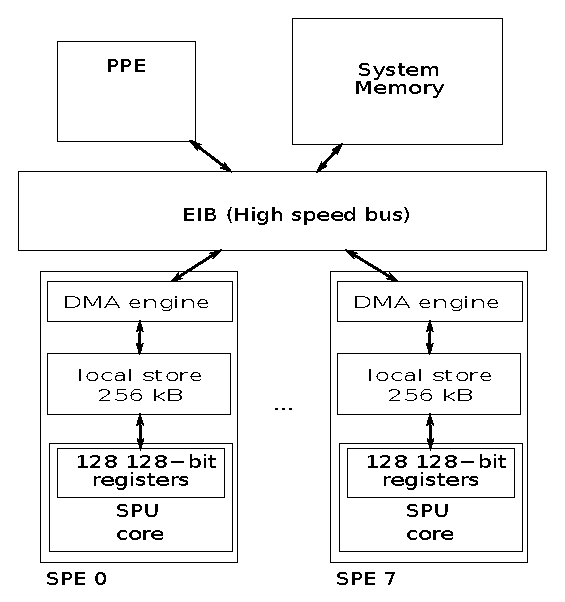
\includegraphics[width=10cm]{data/cellLayout.eps}
    \caption[CellBE processor layout]{One PPE unit along with eight SPE stream processor units and system memory connected together with high speed EIB bus}
    \label{fg:processorLayout}
\end{figure}

A number of signal processing and media applications have been implemented on Cell with excellent results. Advanced visualization such as ray-casting, ray-tracing, and volume rendering. Streaming applications such as media encoders and decoders and streaming encryption and decryption standards have also been demonstrated to perform about an order of magnitude better on Cell than on conventional PC.

\subsection{PPE - \text{PowerPC\textregistered} Processing Element}
PPE is derived from IBM \text{PowerPC\textregistered} core. Has 512kB L2 cache in die. It supports the Power Architecture ISA, inherits the memory translation, protection, and SMP coherence model of mainstream 64-bit Power processors. CBEA also supports virtualization (logical partitioning), large pages, and other recent innovations in the Power architecture. Programming for the PPE is the same as for conventional processors.

\subsection{SPU - Synergistic Processing Element}
SPE is an autonomous processor (sometimes called accellerator) targeted for computational intensive applications. It supports a SIMD-RISC instruction set. Has 128 (128-bit long) unified registers to store all types of data (in contrast from traditional RISCs where registers are devided according data types). One of CellBE programming aspects is converting the code that it uses the SIMD instructions. This process is calleed "SIMDation".

SPE stores its program and data in its associated local storage memory as private memory. DMA transactions are used to tranfer data from/to central memory as well as between two local stores. We say that data is "DMAed" from source to destination. DMA commands can be issued in many ways. Synchronous, asynchronous, in scatter-gaether manner through DMA lists. This memory management is another big part of programming for CellBE.

Programming for SPE has some differencies over programming for conventional processor. You have always to count with the fact you have only 256kB for your program and data. Data is 

This processor is embeded in Sony Playstation 3 game console as well as IBM Blade servers where two or more such processors (as building blocks) connected by high speed bus creates powerfull and modular machine. I have PlayStation3 machine available for my work.